\section{Experiments}
brief overview of the experiments/models

\subsection{Random forest}
% https://www.tensorflow.org/decision_forests
TensorFlow Decision Forests (TF-DF) is the library used to train and evaluate the random forest model.

% (https://www.stat.berkeley.edu/~breiman/randomforest2001.pdf)
A Random Forest is a collection of deep CART decision trees trained independently and without pruning.
Each tree is trained on a random subset of the original training dataset (sampled with replacement).
The algorithm is unique in that it is robust to overfitting, even in extreme cases e.g. when there are more features than training examples.
It is probably the most well-known of the Decision Forest training algorithms.

\subsubsection{Features}
We need to adjust the dataset because the Random Forest model does not accept time series or multivariate data as input.

\begin{figure}[!htbp]
  \begin{subfigure}{.5\textwidth}
    \centering
    \[
      \begin{blockarray}{ccccc}
        & b_0 & b_1 & \dots & b_{15} \\
        \begin{block}{c|cccc|}
          t_0 & 0.2 & 1.6 & \dots & 1.7  \\
          t_1 & 1.3 & 1.8 & \dots & 1.8 \\
          \vdots & \vdots & \vdots &  & \vdots   \\
          t_{53} & 0.6 & 0.4 & \dots & 1.3 \\
        \end{block}
      \end{blockarray}
    \]
    \caption{One observation in a 2-dim array}
    \label{fig:figtrans1}
  \end{subfigure}%
  \begin{subfigure}{.5\textwidth}
    \centering
    \[
      \begin{blockarray}{cc}
      \begin{block}{c|c|}
        t_0::b_0 & 0.2 \\
        t_0::b_1 & 1.6 \\
        \vdots & \vdots \\
        t_{53}::b_{15} & 1.3 \\
      \end{block}
      \end{blockarray}
    \]
    \caption{Forged features for Random forest}
    \label{fig:figtrans2}
  \end{subfigure}
  \caption{Transformation of one observation from a 2-dim array to a 1-dim array}
  \label{fig:figtrans}
\end{figure}

As shown in Figure \ref{fig:figtrans1}, each sample is initially represented by a 2-dimensional array of size (54, 16), where 16 bands capture the pixel's characteristics and 54 time steps reflect its progression. 
However, through the transformation process, the representation is transformed into a more 1-dimensional array of size (864, 1) as depicted in Figure \ref{fig:figtrans2}. 

The model's training utilizes the new representation of the data, composed of 864 derived features, to generate 300 trees.
The performance of each tree is then summarized in Table \ref{tab:rfresults}, which displays the number of nodes, the number of features utilized, and the overall accuracy

\begin{table}[!htbp]
  \centering
    \begin{tabular}{lrrr}
    Model                       & Nodes   & Used features & Overall Accuracy             \\[0.2cm] 
    \hline \\[-0.2cm]
    Imputed missing values      & 523,636  & 753          & $91.03 \pm 0.42$\\
    Not imputed missing values  & 519,932  & 718          & $89.72 \pm 0.84$
    \end{tabular}
  \caption{Random forest results}
  \label{tab:rfresults}
\end{table}


\subsection{TempCNN}
%- paper overview

``Temporal Convolutional Neural Network for the Classification of Satellite Image Time Series'' article \cite{tempCNN} presents a machine learning model for classifying satellite image time series data.
The model is based on Convolutional Neural Networks (CNNs) and aims to improve upon traditional image classification methods by incorporating time-series information into the model.

% - tell that we used the model for the experiments
The Temporal Convolutional Neural Network (TempCNN) architecture was utilized in the following experiments to classify satellite image time series.


The model inputs a series of satellite images and applies a series of convolutional and pooling operations to extract high-level features from the data.
The article introduces a novel approach to classifying satellite image time series data and highlights the potential applications of the model in fields such as remote sensing and environmental monitoring.

\subsubsection{Temporal Convolutions}
% - TODO review
Convolutional layers have been proposed to limit the number of weights a network needs to learn, while trying to make the most of the structuring dimensions in the data, e.g. spatial, temporal or spectral-\cite{NIPS1989_53c3bce6}.
They apply a convolution filter to the output of the previous layer. As compared to dense layers (i.e., the fully-connected layer presented in Section 2.1) where the output of a neuron is a single number reflecting the activation, the output of a convolution filter is an activation map. 
For example, if the input is a univariate time series, then the output will be a time series where each point in the series is the result of the convolution filter.

Convolutional layers have the peculiarity of sharing their parameters across different locations: the same linear combination is applied by sliding it over the entire input.
This drastically reduces the number of weights in the layer, by assuming that the same convolution might be useful in different parts of the time series.
Therefore, the number of trainable parameters depends only on the filter size of the convolution $f$ and the number of units n, but not on the size of the input.
Conversely, the size of the output will depend on the size of the input, and also on two other hyper-parameters—the stride and the padding.
The stride represents the interval between two convolution centers.
Padding controls the addition of values (usually zeros) at the start and end of the input series, before the calculation of the convolution.
It makes it possible, for instance, to ensure that the output has the same size as the input.

\subsubsection{Data preparation}

The dataset was divided into three subsets: training (60\%), validation (20\%), and test (20\%).
To prevent spatial autocorrelation, we ensured that pixels from the same polygon did not appear in different sets.
We also maintained the similarity of class distribution in each set by keeping the same proportions of classes in the training, validation, and test sets.

% TODO: z-normalization?
To normalize the data, we used min-max normalization, the same used in \cite{tempCNN}.
The traditional min-max normalization performs a subtraction of the minimum, then a division by the range, i.e., the maximum minus the minimum \cite{han2011data}.
This normalization is highly sensitive to extreme values, we propose to use 2\% (or 98\%) percentile rather than the minimum (or the maximum) value. 
For each feature, both percentile values are extracted from all the time-stamp values.


\subsubsection{Model}

The baseline architecture of TempCNN used for the experiments as shown in Figure \ref{tab:temCNNArchitecture} consists of three convolutional layers (64 units), one dense layer (256 units) and one softmax layer.
In the experimental section we will investigate the width (i.e. number of units) of the convolutional layers and the depth (i.e. number of convolutional layers) of the network.

\begin{figure}[!htbp]
  \centering
  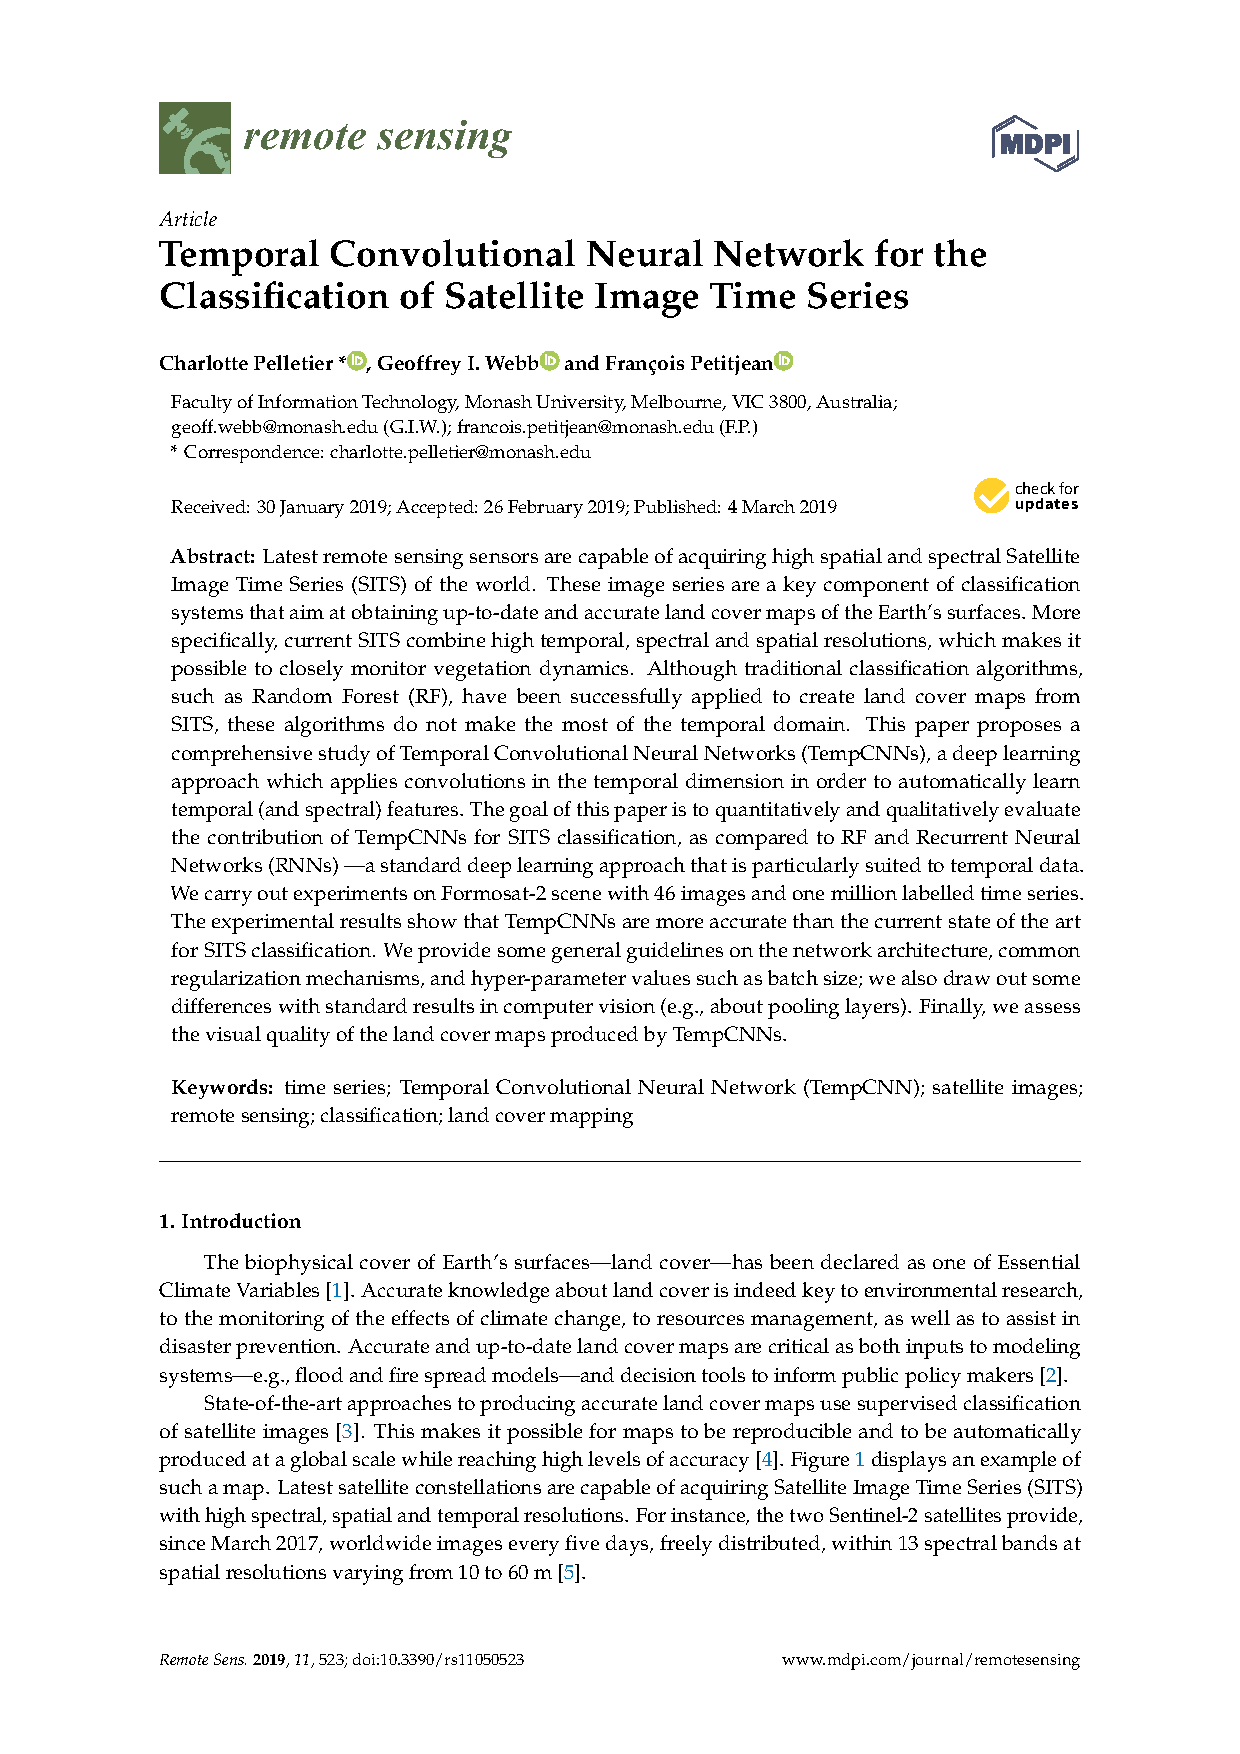
\includegraphics[width=1\textwidth]{tempCNN}
  \caption{Proposed temporal Convolutional Neural Network (TempCNN). The network input is a
  multi-variate time series. Three convolutional filters are consecutively applied, then one dense layer,
  and finally the Softmax layer, that provides the predicting class distribution.    \cite{tempCNN}}
  \label{tab:temCNNArchitecture}
\end{figure}


To prevent overfitting, we employed the same regularization mechanisms described in \cite{tempCNN}:

\begin{itemize}
  \item dropout rate of 0.5 \cite{JMLR:v15:srivastava14a}. 
  \item L2-regularization on the weights (also named weight-decay) applied for all the layers with a small rate of $10^{-6}$ 
  \item batch normalisation \cite{DBLP:journals/corr/IoffeS15}.
\end{itemize}

To train the network Adam optimization was used with the standard parameter values: $\beta_1 = 0.9$, $\beta_2 = 0.999$, and $e = 10^{-8}$) \cite{kingma2014adam} 
We used a batch size of 32, and a maximum number of epochs set to 20, with an early stopping mechanism with a patience of zero on the validation loss. 



- filter size
-- guidance

\subsubsection{Experimental results}

In this section, we report the results of our experiments evaluating the performance of the TempCNN model on satellite image time series data.
We analyzed the effect of the depth of the network and the width of its convolutional layers on the classification accuracy.
Additionally, we investigated the effect of using different regularization techniques on the classification accuracy.
Finally, we investigated the effect of batch size on classification accuracy. 
By thoroughly investigating these factors, we gained insight into how to optimize the TempCNN model for this type of data.


\begin{paragraph}{Depth}
In a convolutional neural network (CNN), the depth refers to the number of layers in the network.
A deeper network can learn more complex features by using a hierarchy of layers, each building on the features learned by the previous layer.
However, increasing the depth can also lead to the vanishing gradient problem, where the gradients become too small to effectively update the weights during training.
Therefore, finding the optimal depth is a crucial consideration when designing a CNN.
\end{paragraph}

To investigate the impact of network depth on model performance while maintaining constant complexity, we vary the number of layers in the network while reducing the number of units in deeper layers.
We experiment with six architectures that consist of between one and six convolutional layers, each with a varying number of units ranging from 256 to 16.
Additionally, each architecture includes one dense layer with a number of units ranging from 64 to 2048. 
In each experiment, we train the model twice: first using the dataset with pre-imputed missing values, and then using a modified dataset where any missing values are replaced with zeros.
As shown in Table \ref{tab:temCNNdepth}, the highest accuracy is achieved with two or three convolutional layers.

\begin{table}[!htbp]
  \centering
   \begin{tabular}{rclrr}
   Model&&                  & No imputation         & Pre imputation             \\[0.2cm]
   \hline \\[-0.2cm]
    1CONV256 &+& 1FC64   	 & $90.01 \pm 0.97$ 	 & $90.80 \pm 0.65$\\
    2CONV128 &+& 1FC128  	 & $\mathbf{93.50 \pm 1.81}$ 	 & $\mathbf{92.97 \pm 2.05}$\\
    3CONV64 &+& 1FC256   	 & $93.45 \pm 1.36$ 	 & $91.29 \pm 1.18$\\
    4CONV32 &+& 1FC512   	 & $91.89 \pm 2.10$ 	 & $88.94 \pm 1.34$\\
    5CONV16 &+& 1FC1024  	 & $90.66 \pm 1.21$ 	 & $86.54 \pm 2.00$\\
    6CONV8 &+& 1FC2048   	 & $86.74 \pm 3.71$ 	 & $87.95 \pm 2.22$\\
   \end{tabular}
   \caption{Influence of depth on classification accuracy.}
   \label{tab:temCNNdepth}
 \end{table}

\begin{paragraph}{Width}
The width of a convolutional neural network (CNN) refers to the number of neurons in each layer.
Increasing the width can enhance the network's ability to learn complex features because more neurons are available for training.
However, a network that is too wide may be prone to overfitting, where it memorizes the training data rather than generalizing to new data.
Therefore, finding the optimal width is critical for achieving the best performance on the test data.
\end{paragraph}

% TODO wainting for results with 2CONV
To evaluate the impact of width on model performance, we experimented with seven CNN architectures.
Each architecture includes three convolutional layers, one dense layer with 256 neurons, and a Softmax layer, as illustrated in Figure \ref{tab:temCNNwidth}.
The architectures differ in the number of parameters, and we vary the width of the convolutional layers from 16 to 1024 neurons.

% describe table below
% - we need something samll because we have a small dataset with few labels

% TODO table may change
 \begin{table}[!htbp]
  \centering
   \begin{tabular}{rclrr}
   Model&&                  & No imputation         & Pre imputation             \\[0.2cm]
   \hline \\[-0.2cm]
    3CONV16 &+& 1FC256    	 & $92.64 \pm 0.01$ 	 & $91.69 \pm 0.12$\\
    3CONV32 &+& 1FC256    	 & $\mathbf{93.88 \pm 0.76}$ 	 & $91.78 \pm 0.53$\\
    3CONV64 &+& 1FC256    	 & $92.48 \pm 2.01$ 	 & $92.72 \pm 0.38$\\
    3CONV256 &+& 1FC256   	 & $91.32 \pm 3.22$ 	 & $91.47 \pm 0.51$\\
    3CONV512 &+& 1FC256   	 & $90.96 \pm 5.13$ 	 & $92.40 \pm 0.70$\\
    3CONV1024 &+& 1FC256  	 & $92.87 \pm 2.33$ 	 & $\mathbf{93.40 \pm 0.37}$\\
   \end{tabular}
   \caption{Influence of width on classification accuracy.}
   \label{tab:temCNNwidth}
 \end{table}




 
- batch-size

\begin{table}[!htbp]
  \centering
   \begin{tabular}{lrr}
   batchsize                  & No imputation         & Pre imputation             \\[0.2cm]
   \hline \\[-0.2cm]
    16  	 & $91.92 \pm 1.50$ 	 & $92.16 \pm 2.75$\\
    32  	 & $\mathbf{91.61 \pm 1.99}$ 	 & $\mathbf{93.74 \pm 0.03}$\\
    64  	 & $90.88 \pm 2.63$ 	 & $92.30 \pm 2.89$\\
    128  	 & $91.54 \pm 2.99$ 	 & $91.52 \pm 1.67$\\
   \end{tabular}
   \caption{batchsize 3CONV64+1FC256}
 \end{table}

 \begin{table}[!htbp]
  \centering
   \begin{tabular}{lrr}
   Model                  & No imputation         & Pre imputation             \\[0.2cm]
   \hline \\[-0.2cm]
    
  
    3CONV64C + 1FC256 + GAP + f33  	 & $91.45 \pm 0.86$ 	 & $90.01 \pm 0.81$\\
    3CONV64C + 1FC256 + GAP + f17  	 & $90.43 \pm 3.00$ 	 & $90.10 \pm 4.35$\\
    3CONV64C + 1FC256 + GAP + f9  	 & $90.09 \pm 1.62$ 	 & $90.22 \pm 0.25$\\
    3CONV64C + 1FC256 + GAP + f5  	 & $91.41 \pm 0.12$ 	 & $88.13 \pm 5.74$\\
    3CONV64C + 1FC256 + GAP + f3  	 & $89.61 \pm 3.55$ 	 & $91.10 \pm 0.08$
    \\[0.2cm] \hline \\[-0.2cm]
    3CONV2MP + 1FC256 + f33 + 17 + 9  	 & $92.10 \pm 1.87$ 	 & $89.73 \pm 2.23$\\
    3CONV2MP + 1FC256 + f17 + 9 + 5  	 & $89.35 \pm 0.55$ 	 & $89.11 \pm 3.84$\\
    3CONV2MP + 1FC256 + f9 + 5 + 3  	 & $91.23 \pm 4.56$ 	 & $91.33 \pm 1.52$\\
    3CONV2MP + 1FC256 + f5 + 3 + 1,  	 & $91.71 \pm 3.48$ 	 & $93.07 \pm 0.87$\\
    3CONV2MP + 1FC256 + f3 + 1 + 1,  	 & $93.10 \pm 3.08$ 	 & $91.45 \pm 0.06$
    \\[0.2cm] \hline \\[-0.2cm]
    3CONV2AP + 1FC256 + f33 + 17 + 9  	 & $90.41 \pm 2.94$ 	 & $91.45 \pm 1.15$\\
    3CONV2AP + 1FC256 + f17 + 9 + 5  	 & $93.61 \pm 0.23$ 	 & $92.78 \pm 1.51$\\
    3CONV2AP + 1FC256 + f9 + 5 + 3  	 & $91.56 \pm 0.81$ 	 & $86.86 \pm 8.06$\\
    3CONV2AP + 1FC256 + f5 + 3 + 1,  	 & $92.72 \pm 0.34$ 	 & $92.23 \pm 2.47$\\
    3CONV2AP + 1FC256 + f3 + 1 + 1,  	 & $93.71 \pm 0.61$ 	 & $92.74 \pm 1.26$
    \\[0.2cm] \hline \\[-0.2cm]
    3CONV2MP + 1FC256 + GAP + f33 + 17 + 9  	 & $91.10 \pm 1.39$ 	 & $90.75 \pm 0.55$\\
    3CONV2MP + 1FC256 + GAP + f17 + 9 + 5  	 & $91.20 \pm 1.38$ 	 & $91.05 \pm 0.56$\\
    3CONV2MP + 1FC256 + GAP + f9 + 5 + 3  	 & $90.15 \pm 1.41$ 	 & $92.37 \pm 0.65$\\
    3CONV2MP + 1FC256 + GAP + f5 + 3 + 1,  	 & $91.90 \pm 0.45$ 	 & $89.69 \pm 2.57$\\
    3CONV2MP + 1FC256 + GAP + f3 + 1 + 1,  	 & $90.76 \pm 3.19$ 	 & $89.32 \pm 2.65$
    \\[0.2cm] \hline \\[-0.2cm]
    3CONV2AP + 1FC256 + GAP + f33 + 17 + 9  	 & $86.05 \pm 5.55$ 	 & $91.16 \pm 0.47$\\
    3CONV2AP + 1FC256 + GAP + f17 + 9 + 5  	 & $89.74 \pm 2.89$ 	 & $91.74 \pm 2.30$\\
    3CONV2AP + 1FC256 + GAP + f9 + 5 + 3  	 & $91.35 \pm 0.53$ 	 & $92.49 \pm 0.36$\\
    3CONV2AP + 1FC256 + GAP + f5 + 3 + 1,  	 & $90.17 \pm 1.79$ 	 & $91.64 \pm 2.40$\\
    3CONV2AP + 1FC256 + GAP + f3 + 1 + 1  	 & $90.59 \pm 3.77$ 	 & $90.61 \pm 1.05$\\
   \end{tabular}
   \caption{pooling}
 \end{table}
 

\pagebreak
\subsection{AJ-RNN}
- model overview

- GRU vs LSTM (running)

- learnig rate
- batch size 

\subsubsection{Light AJ-RNN}
- model overview\\
- baseline

\subsection{L-TAE}
- model overview\\
- PixelSetEncoder\\
- DenseEncoder

- imputation vs no imputation
- tanh

\subsection{Results}

\begin{table}[!htbp]
  \centering
    \begin{tabular}{lrrr}
    Model                       & Overall Accuracy             \\[0.2cm] 
    \hline \\[-0.2cm]
    RF      & $91.03 \pm 0.42$
    \end{tabular}
  \caption{Overall accuracy of the models with pre imputed missing values} 
\end{table}

\begin{table}[!htbp]
  \centering
    \begin{tabular}{lrrr}
    Model                       & Overall Accuracy             \\[0.2cm] 
    \hline \\[-0.2cm]
    RF  & $89.72 \pm 0.84$
    \end{tabular}
  \caption{Overall accuracy of the models with missing values} 
\end{table}